%##############################################
\chapter{The standard model of particle physics}
%##############################################

\intro{In the following an overview of the \gls{sm} is given. First, the fundamental particles and their properties are introduced. Then the electroweak and strong interactions are detailed which includes a brief descriptions of the electroweak symmetry breaking mechanism as well. After sketching the calculation of observables in perturbative theory the chapter is concluded by highlighting some open questions of the \gls{sm}.}

The \gls{sm} describes the interactions between fundamental particles. It is based on \gls{qft} which allows to predict observables of particle interactions. Exemplary observables are production cross sections or decay rates of particles which can be calculated within its framework. The \gls{sm} validity is constantly challenged by comparing predictions to experimental data. No significant deviations have been found so far that would hint towards \gls{bsm} physics.


%############################################## 
\section{Particle content}
%##############################################

Fundamental particles are defined as objects for which experiments have not revealed an internal structure. For example, the upper limit on the spatial radius of the electron is measured to be $<10^{-18}~\mathrm{m}$~\cite{PhysRevLett.97.030801}. Hence, such fundamental particles are considered as point-like. They can be grouped by their spin into fermions with half-integer and bosons with integer spin. All fundamental fermions of the \gls{sm} have a spin of $\frac{1}{2}$. They can be further divided into leptons and quarks where only the latter can participate in strong interactions. Tables~\ref{tab:theory-leptons} and~\ref{tab:theory-quarks} list the leptons and quarks respectively. Each column is called a generation. It encapsulates an isospin pair whose components are therefore also referred to as up- or down-type respectively. It is unknown why there are exactly three lepton and three quark generations. Atoms which form ordinary matter consist of only particles from the first generation: electrons, protons, and neutrons, where the latter two are bound states of uud quarks and udd quarks respectively.

\mytable{\label{tab:theory-leptons}Leptons of the \gls{sm}. Particle masses are taken from Ref.~\cite{Olive:2016xmw}. Uncertainties on the measured masses are omitted because the precision is beyond the sub permille level. For the neutrino masses only \glspl{cl} are given.}{
    \begin{tabular}{|r|c c c|}
    \hline
                        & 1. generation                 & 2. generation                 & 3. generation \\
    \hline
    \hline
    name                & electron neutrino             & muon neutrino                 & tau neutrino  \\
                        & ($\nu_\mathrm{e}$)            & ($\nu_{\mu}$)                 & ($\nu_{\tau}$) \\
    
    mass                & $<225~\eV$                    & $<0.19~\MeV$                  & $<18.2~\MeV$ \\
                        & (95\% CL)                     & (90\% CL)                     & (95\%~CL)\\
    
    electric charge     & 0                             & 0                             & 0 \\
    \hline
    name                & electron                      & muon                          & tau  \\
                        & ($\mathrm{e}^{\rmminus}$)     & ($\mu^{\rmminus}$)            & ($\tau^{\rmminus}$) \\
    
    mass                & $511.0~\keV$                  & $105.66~\MeV$                 & $1.776~\GeV$ \\
                        &                               &                               &  \\
    electric charge     & $-1$                          & $-1$                          & $-1$ \\
    \hline
    \end{tabular}
}

For the masses of the neutrinos, only upper limits are set. Those are derived by combining measurements of beta decay spectra with results from neutrino oscillation experiments. When the \gls{sm} was constructed in the mid 1970s, the neutrinos were assumed to be massless. However, the observation of neutrino oscillations requires that at least two neutrinos have a non-zero mass~\cite{Fukuda:1998mi}.

\mytable{\label{tab:theory-quarks}Quarks of the \gls{sm}. For u,d,s,c,b quarks \gls{msbar} masses are quoted, taken from Ref.~\cite{Olive:2016xmw}. The top quark pole mass is taken from Ref.~\cite{Khachatryan:2015hba}.}{
\begin{tabular}{|r|c c c|}
    \hline
                        & 1. generation                 & 2. generation                 & 3. generation \\
    \hline
    \hline
    name                & up (u)                        & charm (c)                     & top (t) \\
    
    mass                & $2.2^{+0.6}_{-0.4}~\MeV$      & $1.27\pm0.03~\GeV$            & $172.44\pm0.49~\GeV$ \\
    
    electric charge     & $\frac{2}{3}$                 & $\frac{2}{3}$                 & $\frac{2}{3}$ \\
    
    \hline
    name                & down (d)                      & strange (s)                   & bottom (b)  \\
    
    mass                & $4.7^{+0.5}_{-0.4}~\MeV$      & $96^{+8}_{-4}~\MeV$           & $4.18^{+0.04}_{-0.03}~\GeV$ \\
    
    electric charge     & $-\frac{1}{3}$                & $-\frac{1}{3}$                & $-\frac{1}{3}$ \\
    \hline
    \end{tabular}
}


The bosons are connected to fundamental interactions by requiring invariance under a gauge group transformation as explained later in this chapter. They are listed in Tab.~\ref{tab:theory-bosons}. All bosons, except the Higgs boson, carry a spin of~$1$. The Higgs boson is the only scalar fundamental particle~(spin~$0$) of the \gls{sm}. For a long time, it was a purely hypothetical particle. In July 2012, the ATLAS~\cite{Aad:2012tfa} and CMS~\cite{Chatrchyan:2012xdj} collaborations independently reported an observation of a Higgs-like particle. Further investigations whether this new particle exhibits the expected interactions with other particles revealed that it is consistent with the \gls{sm} Higgs boson~\cite{Khachatryan:2016vau}. This discovery completed the \gls{sm} and thus gave further confidence into its theoretical foundation.


\mytable{\label{tab:theory-bosons}Bosons of the \gls{sm}. Z and W boson masses are taken from Ref.~\cite{Olive:2016xmw}. The uncertainties on their masses are omitted because the precision is beyond the sub permille level. The Higgs mass is taken from Ref.~\cite{Aad:2015zhl}.}{
\begin{tabular}{|r|c c c|}
    \hline
    name                & mass                 & associated interaction             & gauge group \\
    \hline
    \hline
    photon (\photon)    & $0$                  & electromagnetism                   & $\mathrm{U(1)}$ \\
    
    Z boson (\zboson)   & $91.19~\GeV$         & \multirow{2}{*}{$\Big\}$ weak interaction}  & \multirow{2}{*}{$\mathrm{SU(2)}$}\\
    W boson (\wboson)   & $80.39~\GeV$         &                                    & \\
    
    Higgs boson (\higgs)& $125.09\pm0.24~\GeV$ & Yukawa interaction                 & $\mathrm{SU(2)}\otimes\mathrm{U(1)}$\\
      
    8 gluons (g)        & $0$                  & strong interaction                 & $\mathrm{SU(3)}$ \\  
    \hline               
    \end{tabular}
}

For each fundamental particle there exists a charge-conjugated partner called antiparticle. Other properties such as mass are identical. The photon, Z boson, and Higgs boson are their own antiparticle. It is still under investigation if the neutrino is its own antiparticle. Fermions with such a property are called Majorana particles~\cite{Majorana2006}. Experimentally, this can be probed in double $\beta$ decays~($\mathrm{nn}\to\mathrm{pp}+\mathrm{e}^{\rmminus}\mathrm{e}^{\rmminus}\nu_\mathrm{e}\nu_\mathrm{e}$) where in the case of Majorana neutrinos the decay can occur without emitting two neutrinos. However, this scenario seems to be disfavored by recent results as reviewed in Ref.~\cite{Dell'Oro:2016dbc}.


%##############################################
\section{Quantum field theory}
%##############################################

In the framework of \gls{qft}, particles are described as excitation modes of quantized fields. This is also referred to as ``second quantization'' allowing to describe the dynamics of many-particle systems. Field operators can be decomposed as

\begin{align}
    \hat{\psi}(x)&=\sum_{i}^{\mathrm{N}}u_{i}(x)\hat{a}_{i} \\
    \hat{\psi}^{\dagger}(x)&=\sum_{i}^{\mathrm{N}}u^{\star}_{i}(x)\hat{a}^{\dagger}_{i},
\end{align}

where $u_{i}(x)$ denotes the ordinary wave function of a single particle and $\hat{a}^{\dagger}_{i}$ ($\hat{a}_{i}$) its creation (annihilation) operator, respectively.

As in classical mechanics, the action of a system can be expressed as

\begin{equation}
S=\int\mathrm{L}\,\mathrm{d}t=\iint\mathcal{L}\,\mathrm{d}^{3}\vec{x}\,\mathrm{dt}=\int\mathcal{L}\,\mathrm{d}^{4}x
\end{equation}

with the Lagrangian density $\mathcal{L}$. For example, a system of free fermions is described by the Dirac Lagrangian density,

\begin{equation}
\label{eq:theory-diracL}
\mathcal{L}_\mathrm{Dirac}=\bar{\psi}\big(i\gamma^\mu\partial_\mu-m\big)\psi
\end{equation}

using the definitions $\partial_\mu\equiv\partial/\partial x_\mu$ and $\bar{\psi}\equiv\psi^\dagger\gamma^{0}$ where $\gamma_\mu$ denote the Dirac matrices\footnote{Multiple representations are possible. The matrices need to satisfy a Clifford algebra with the anticommutation relation: $\big\{\gamma^\mu,\gamma^\nu\big\}=\gamma^\mu\gamma^\nu+\gamma^\nu\gamma^\mu=2g^{\mu\nu}$.}. The principle of least action, $\delta \mathrm{S}=0$, that is satisfied by the Euler-Lagrange equation yields the equation of motion as

\begin{equation}
\frac{\partial\mathcal{L}}{\partial\bar{\psi}}-\frac{\partial}{\partial_\mu}\Bigg(\frac{\partial\mathcal{L}}{\partial\big(\partial_\mu\bar{\psi}\big)}\Bigg)=\big(i\gamma^\mu\partial_\mu-m\big)\psi=0. \\
\end{equation}

In the \gls{sm}, interactions between particles are introduced by requiring local invariance of the Lagrangian density for certain groups of gauge transformations. In the following, this is briefly demonstrated for the case of a $\mathrm{U(1)}$ transformation which leads to electromagnetic interactions.

The transformation of Eq.~\ref{eq:theory-diracL} using 

\begin{equation}
\psi(x)\mapsto\psi^{\prime}(x)=\psi\exp^{-iq\alpha(x)}
\end{equation}

where the phase $\alpha(x)$ depends on the local coordinates $x$ yields

\begin{equation}
\mathcal{L}(\psi,\partial_\mu\psi)\mapsto\mathcal{L}(\psi^{\prime},\partial_\mu\psi^{\prime})=\bar{\psi}\big(i\gamma^\mu\partial_\mu+q\gamma^\mu\partial_\mu\alpha(x)-m\big)\psi.
\end{equation}

The invariance $\mathcal{L}(\psi,\partial_\mu\psi)=\mathcal{L}(\psi^{\prime},\partial_\mu\psi^{\prime})$ is restored by adding a bosonic spin-1 field $\mathrm{A}_{\mu}(x)$ which interacts with $\psi$ while transforming as

\begin{equation}
\mathrm{A}_{\mu}(x)\mapsto \mathrm{A}^{\prime}_{\mu}(x)=\mathrm{A}_\mu(x)-\partial_\mu\alpha(x).
\end{equation}

This procedure yields a Lagrangian density containing the following terms:

\begin{align}
\mathcal{L}=~~&\bar{\psi}\big(i\gamma^\mu\partial_\mu-m\big)\psi &(\mathrm{fermion~propagator}) \\
            +&q\bar{\psi}\gamma^{\mu}\psi \mathrm{A}_{\mu} &(\mathrm{interaction}) \label{eq:theory-EM-int}\\
            -&\tfrac{1}{4}\big(\partial_\mu \mathrm{A}_\nu-\partial_\nu \mathrm{A}_\mu\big)^{2} &(\mathrm{boson~propagator})
\end{align}

In addition, the already gauge-invariant boson propagator describing the dynamics of a free $\mathrm{A}_\mu$ field has been added. The introduced interaction~(Eq.~\ref{eq:theory-EM-int}) which is required to ensure the invariance under $\mathrm{U(1)}$ transformation can be identified as electromagnetic interaction between a fermion described by $\psi$ with electric charge $q$ and a photon described by $\mathrm{A}_\mu$. Furthermore, the photon is predicted to be massless since adding a term of the form $m^{2}_\mathrm{A}\mathrm{A}^\mu \mathrm{A}_\mu$ would violate the invariance.

Other interactions of the \gls{sm} are also connected to local gauge transformations which can be introduced through similar procedures. A common property follows from the Noether theorem which states that for each continuous transformation a conserved current exists. Hence the charge associated to each gauge group is conserved. This would however be already the case for a global transformation. The invariance under an even local gauge transformations is a puzzling feature of the theory.



%##############################################
\section{Electroweak interactions and Higgs mechanism}
%##############################################
\label{sec:theory-ewk}

Electromagnetic and weak interactions can be unified using a $\mathrm{U(1)}\otimes \mathrm{SU(2)}$ gauge group. A complication arises from the fact that the $\mathrm{W}$~and $\mathrm{Z}$~bosons, mediatiors of the weak interaction, are massive. The masses of these particles have to be introduced in a different way if the concept of local gauge invariance should continue to hold. Experimentally, the UA1 and UA2 experiments at the \gls{cern} \gls{sps} proton-antiproton collider measured their masses for the first time~\cite{Arnison:1983rp,Banner:1983jy,Arnison:1983mk,Bagnaia:1983zx} while their existence was already known from bubble chamber experiments\todo{what ???}.

Another feature of weak interactions is that parity is not conserved but maximally violated. The interaction depends on the spin being aligned towards or against the momentum of a particle. Experimentally, the Wu experiment~\cite{PhysRev.105.1413} discovered this feature in ${}_{27}^{60}\mathrm{Co}\to{}_{28}^{60}\mathrm{Ni}+e^{\rmminus}\bar{\nu}_{e}\gamma\gamma$ decays by analyzing the direction of the escaping electron with respect to the polarization of the cobalt probe through an external magnetic field. To account for the violation of parity, fermion fields are decomposed into chiral eigenstates using the projections

\begin{align}
\psi_\mathrm{L}&\equiv\mathrm{P}_\mathrm{L}\psi=\tfrac{1}{2}(1-\gamma_{5})\psi \\
\psi_\mathrm{R}&\equiv\mathrm{P}_\mathrm{R}\psi=\tfrac{1}{2}(1+\gamma_{5})\psi
\end{align}

with $\gamma_{5}=i\gamma_{0}\gamma_{1}\gamma_{2}\gamma_{3}$\footnote{Properties: $(\gamma_{5})^{\dagger}=\gamma_{5}$; ~~$(\gamma_{5})^2=\mathrm{I}_\mathrm{4x4}$; ~~ $\{\gamma_{5},\gamma_{\mu}\}=\gamma_{5}\gamma_{\mu}+\gamma_{\mu}\gamma_{5}=0$.} where $\psi_\mathrm{L}$ ($\psi_\mathrm{R}$) is called a ``left-handed'' (``right-handed'') fermion respectively. In the case of massless particles, Eq.~\ref{eq:theory-diracL} decouples into two independent equations for $\psi_\mathrm{L}$ and $\psi_\mathrm{R}$. In such a case, the chirality would be equal to the Lorentz-invariant helicity

\begin{equation}
H=\frac{\vec{p}\cdot\vec{s}}{|\vec{p}|}
\end{equation}

which denotes whether the spin $\vec{s}$ is aligned along~($H=+1$) or against~($H=-1$) the momentum axis. For massive particles however Eq.~\ref{eq:theory-diracL} cannot be decomposed since chirality is not Lorentz invariant.

In the Glashow-Weinberg-Salam model~\cite{Salam:1964ry,Weinberg:1967tq,Glashow:1961tr} the fermion fields are split into ``left-handed'' doublets 

\begin{align}
\vec{\mathrm{E}}_\mathrm{L}&=\Bigg\{\colvec{2}{\nu_\mathrm{e,L}}{e^{\rmminus}_\mathrm{L}},\colvec{2}{\nu_{\mu,\mathrm{L}}}{\mu^{\rmminus}_\mathrm{L}},\colvec{2}{\nu_{\tau,\mathrm{L}}}{\tau^{\rmminus}_\mathrm{L}}\Bigg\} \label{eq:theory-su2-leptons} \\
\vec{\mathrm{Q}}_\mathrm{L}&=\Bigg\{\colvec{2}{\mathrm{u}_\mathrm{L}}{\mathrm{d}_\mathrm{L}},\colvec{2}{\mathrm{c}_\mathrm{L}}{\mathrm{s}_\mathrm{L}},\colvec{2}{\mathrm{t}_\mathrm{L}}{\mathrm{b}_\mathrm{L}}\Bigg\} \label{eq:theory-su2-quarks}
\end{align}

and ``right-handed'' singlets 

\begin{align}
\vec{\mathrm{e}}_\mathrm{R}=\big\{\mathrm{e}^{\rmminus}_\mathrm{R},\mu^{\rmminus}_\mathrm{R},\tau^{\rmminus}_\mathrm{R}\big\},\quad\vec{\mathrm{u}}_\mathrm{R}=\big\{\mathrm{u}_\mathrm{R},\mathrm{c}_\mathrm{R},\mathrm{t}_\mathrm{R}\big\},\quad\vec{\mathrm{d}}_\mathrm{R}=\big\{\mathrm{d}_\mathrm{R},\mathrm{s}_\mathrm{R},\mathrm{b}_\mathrm{R}\big\} \label{eq:theory-su2-singlets}
\end{align}

of the $\mathrm{SU(2)}$ group. Right-handed neutrinos do not participate in any interaction within the \gls{sm}. The gauge transformation of the combined $\mathrm{U(1)}\otimes \mathrm{SU(2)}$ group is

\begin{equation}
\psi\mapsto\psi\cdot\mathrm{e}^{-ig\vec{\alpha}(x)\cdot\vec{\omega}/2}\cdot\mathrm{e}^{-ig^{\prime}\beta(x)/2} \label{eq:theory-u1su2-transformation}
\end{equation}

where $\omega_{a}$~($a\in\{1,2,3\}$) denote the Pauli matrices and $g$, $g^{\prime}$ the corresponding conserved charges. This leads to four boson fields, $\mathrm{W}^{a}$ and $\mathrm{B}$, that interact with the fermions. In analogy to Eq.~\ref{eq:theory-EM-int} one obtains

\begin{align}
\mathcal{L}_\mathrm{interaction}=~~\sum_{\psi_\mathrm{L}}^\mathrm{doublets}&\bar{\psi}^{i}_\mathrm{L}~\gamma^{\mu}\big(\tfrac{1}{2}g\vec{\mathrm{W}}_{\mu}\cdot\vec{\omega}+\tfrac{1}{2}g^{\prime}\mathrm{B}_{\mu}\big)\psi^{i}_\mathrm{L} \nonumber\\
+\sum_{\psi^{i}_\mathrm{R}}^\mathrm{singlets}&\bar{\psi}^{i}_\mathrm{R}~\gamma^{\mu}\tfrac{1}{2}g^{\prime}\mathrm{B}_{\mu}\psi^{i}_\mathrm{R} + \mathrm{\gls{hc}} \label{eq:theory-codev-su2-interaction}
\end{align}

where the summation is implied over the fermion doublets and singlets.

A fermion mass term $\propto m_\mathrm{f}\bar{\psi}_\mathrm{f}\psi_\mathrm{f}=m_\mathrm{f}(\bar{\psi}_\mathrm{f,L}\psi_\mathrm{f,R}+\bar{\psi}_\mathrm{f,R}\psi_\mathrm{f,L})$ cannot be added to the Lagrangian density since it is not invariant under $\mathrm{SU(2)}$ transformation. A solution is provided by the Englert-Brout-Higgs-Guralnik-Hagen-Kibble-mechanism~\cite{HIGGS1964132,PhysRevLett.13.508,PhysRevLett.13.321,PhysRevLett.13.585} which introduces mass terms not only for fermions but also for the gauge bosons through symmetry breaking. For this, a new scalar $\mathrm{SU(2)}$ doublet field $\phi=(\phi^{\rmplus},\phi^{0})$\footnote{$\phi^{\rmplus}$ annihilates positively charge scalar particles / creates antiparticles with negative charge; $\phi^{0}$ annihilates neutral particles / creates neutral antiparticles.} (invariant under $\mathrm{U(1)}\otimes\mathrm{SU(2)}$) is added to the Lagrangian density

\begin{align}
\mathcal{L}_{\phi}&=\big(D_{\mu}\phi^{\dagger}\big)\big(D^{\mu}\phi\big)+\mathrm{V}(\phi) \label{eq:theory-phi-propagator} \\
D^{\mu}\phi&=\big(\partial^{\mu}+\tfrac{1}{2}ig\vec{\mathrm{W}}^{\mu}\cdot\vec{\omega}+\tfrac{1}{2}ig^{\prime}\mathrm{B}^{\mu}\big)\phi \label{eq:theory-phi-codev}
\end{align}

which interacts with the gauge bosons. In addition, $\phi$ has a potential 

\begin{equation}
\mathrm{V}(\phi)=-\mu^2\phi^\dagger\phi+\tfrac{1}{2}\lambda(\phi^\dagger\phi)^2
\end{equation}

in the form of a ``Mexican hat'' as shown in Fig.~\ref{fig:theory-higgs-potential} that leads to a \gls{vev} of $\phi_0=\sqrt{\mu^{2}/\lambda}\equiv v/\sqrt{2}$ for $\mu^2>0$.

\myfigure{\label{fig:theory-higgs-potential}The ``Mexican hat'' potential of the Higgs field with a non-zero \gls{vev} $\phi_0$ which leads to symmetry breaking.}{
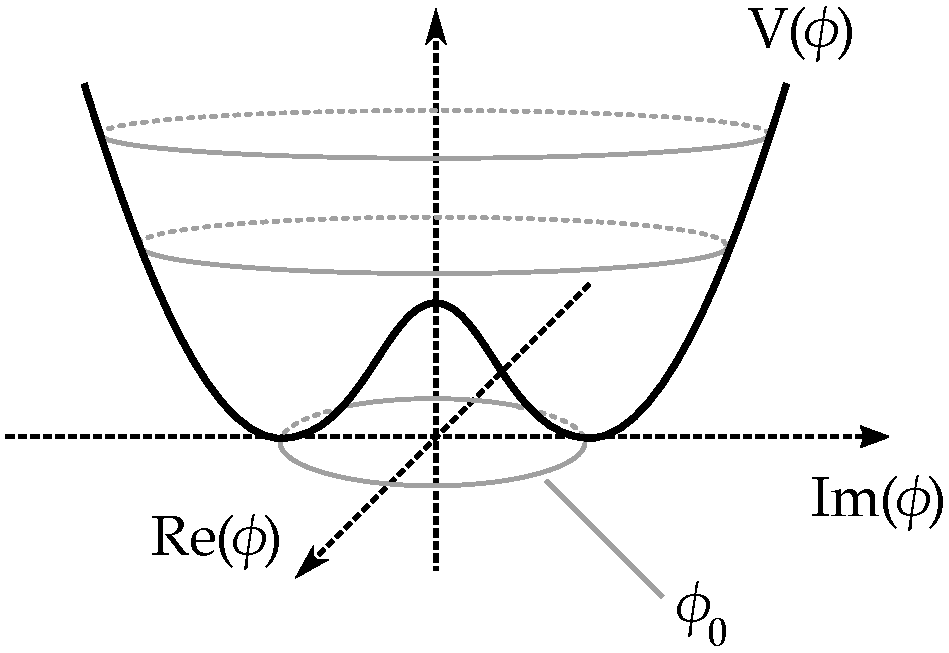
\includegraphics[width=0.5\textwidth]{figures/theory/higgspot.pdf}
}

One says that this shifted \gls{vev} ``breaks'' the $\mathrm{SU(2)}$ symmetry when parameterizing $\phi$ around the minimum as

\begin{equation}
\phi(x) \big|_{\phi_0} = \colvec{2}{0}{\frac{1}{\sqrt{2}}\big(v+\mathrm{H}(x)\big)}\cdot \mathrm{e}^{-i\vec{\theta}(x)\cdot\vec{\omega}/(2v)} \label{eq:theory-phi-dev}
\end{equation}

where $\vec{\theta}$ denotes three so-called ``Goldstone'' bosons and $\mathrm{H}$ the Higgs boson. In fact, the symmetry still exists but is ``hidden''. A $\mathrm{SU(2)}$ transformation (called ``unitary gauge'') can be performed such that $\vec{\theta}$ vanishes. One says that these three Goldstone bosons and their degrees of freedom are ``eaten'' by the $\mathrm{W}$ and $\mathrm{Z}$~bosons to become massive. Hence, they can also have a longitudinal polarization now through the extra degree of freedom. 

After the gauge transformation, only the Higgs boson remains. The parametrization~(Eq.~\ref{eq:theory-phi-dev}) is chosen such that it leaves the minimum of $\phi$ invariant under the $\mathrm{U(1)}$ subgroup transformation

\begin{equation}
\phi\mapsto\phi\cdot\mathrm{e}^{-ig\alpha_{3}(x)\omega_{3}/2}\cdot\mathrm{e}^{-ig^{\prime}\beta(x)/2}. \label{eq:theory-broken-u1-trans}
\end{equation}

Inserting Eq.~\ref{eq:theory-phi-dev} into Eq.~\ref{eq:theory-phi-propagator} yields the following non-interaction terms

\begin{align}
\mathcal{L}_\mathrm{Higgs}=&~~~~\tfrac{1}{2}(\partial_{\mu}\mathrm{H}^{\dagger})(\partial^{\mu}\mathrm{H})-\lambda^2 v^2 \mathrm{H}^2 \label{eq:theory-higgs} \\
\mathcal{L}_\mathrm{W_1,W_2~bosons}=&-\tfrac{1}{4}\big(\mathrm{W}_{1,\mu\nu}\mathrm{W}^{\mu\nu}_{1}+\mathrm{W}_{2,\mu\nu}\mathrm{W}^{\mu\nu}_{2}\big)\nonumber\\&+\tfrac{1}{8}g^2 v^2 \big(\mathrm{W}_{1,\mu} \mathrm{W}_{1}^{\mu}+\mathrm{W}_{2,\mu} \mathrm{W}_{2}^{\mu}\big) \label{eq:theory-a1a2} \\
\mathcal{L}_\mathrm{W_3,B~bosons}=&-\tfrac{1}{4}\big(\mathrm{B}_{\mu\nu}\mathrm{B}^{\mu\nu}+\mathrm{W}_{3,\mu\nu}\mathrm{W}^{\mu\nu}_{3}\big)\nonumber\\&+\tfrac{1}{8}v^2 \big(g\mathrm{W}_{3,\mu}-g^{\prime}\mathrm{B}_\mu\big)\big(g\mathrm{W}_{3}^{\mu}-g^{\prime}\mathrm{B}^\mu\big) \label{eq:theory-a3b}.
\end{align}

The first term (Eq.~\ref{eq:theory-higgs}) describes the free scalar Higgs boson with mass $m_\mathrm{H}=\lambda v$. Next, the $\mathrm{W}_{1}$ and $\mathrm{W}_{2}$
fields in Eq.~\ref{eq:theory-a1a2} can be identified as a particle/antiparticle pair $\mathrm{W}^{\pm}=1/\sqrt{2}(\mathrm{W}_1\mp i\mathrm{W}_2)$ with mass $m_\mathrm{W}=\frac{1}{2}gv$. Lastly, the fields $\mathrm{W}_3$ and $\mathrm{B}$ appear to be in a mixed mass state~(Eq.~\ref{eq:theory-a3b}). By performing a rotation of the couplings

\begin{equation}
\colvec{2}{\mathrm{Z}}{\mathrm{A}}=\begin{pmatrix}
\cos\theta_\mathrm{W} & -\sin\theta_\mathrm{W} \\
\sin\theta_\mathrm{W} & \cos\theta_\mathrm{W}
\end{pmatrix}
\colvec{2}{\mathrm{W}_{3}}{\mathrm{B}},\quad \cos\theta_\mathrm{W}=\frac{g}{\sqrt{g^2+g^{\prime 2}}},
\end{equation}

where $\theta_\mathrm{W}$ is called the ``weak-mixing'' or ``Weinberg'' angle, another massive boson $\mathrm{Z}$~boson with mass $m_\mathrm{Z}=v\sqrt{g^2+g^{\prime2}}/2$ and a massless boson $\mathrm{A}_\mu$, the photon, can be identified. The angle is determined as $\sin^2\theta_\mathrm{W} \approx 0.23$~\cite{Olive:2016xmw} through the mass ratio $m_\mathrm{W}/m_\mathrm{Z}=\cos\theta_\mathrm{W}$.\todo{is the angle determined really this way?} Rewriting the covariant derivative of Eq.~\ref{eq:theory-phi-codev} into these mass eigenstates yields

\begin{align}
D_\mu=&~~~~\partial_\mu+i\frac{g}{\sqrt{2}}\cdot\big(\mathrm{W}^{\rmplus}_\mu T^{\rmplus}+\mathrm{W}^{\rmminus}_\mu T^{\rmminus})\nonumber\\
&-i\frac{g^2T_3-g^{\prime 2}Y}{\sqrt{g^2+g^{\prime 2}}}\cdot\mathrm{Z}_\mu-i\frac{g^{\prime}g\big(T_3+Y\big)}{\sqrt{g^2+g^{\prime 2}}}\cdot \mathrm{A}_\mu \label{eq:theory-codev-breaking}
\end{align}

where $T^{\pm}$ denote the ladder operators, $Y$ the $\mathrm{U(1)}$ so-called ``hyper'' charge and $T_3$ the $\mathrm{SU(2)}$ charge.

From the coupling to the photon one can read off the electric coupling constant to be 

\begin{equation}
e=\frac{g^{\prime} g}{\sqrt{g^2+g^{\prime 2}}}
\end{equation}

which is measured as $\aem=e^2/(4\pi)=1/137$\todo{cite} and the corresponding electric charge to be $Q=T_3+Y$ which is invariant under Eq.~\ref{eq:theory-broken-u1-trans}. For the weak coupling constant one finds the relation $e=g\cdot\sin\theta_\mathrm{W}$ which yields $\aw=\aem/\sin^2\theta_\mathrm{W}\approx0.032$.

In conclusion, starting from a local gauge invariant theory, the procedure of symmetry breaking through a shifted \gls{vev} leads to three Goldstone bosons which are absorbed into mass terms for the $\mathrm{W}$ and $\mathrm{Z}$~bosons. The value of the \gls{vev} can be determined from the Fermi coupling constant, measured in muon decays, as $v\approx 246~\GeV$~\cite{PhysRevLett.106.041803}. Additionally, the existence of the Higgs boson is predicted as consequence of this procedure. It was finally discovered in July 2012 independently by the ATLAS~\cite{Aad:2012tfa} and CMS~\cite{Chatrchyan:2012xdj} collaborations and thus completed the electroweak theory.


The fermion masses can be generated by interacting with the Higgs field as well. One introduces Yukawa interactions as

\begin{align}
\mathcal{L}_\mathrm{Yukawa~lepton~int.}=&-\lambda_{e}^{ii}\cdot\bar{\mathrm{E}}^{i}_\mathrm{L}\phi\cdot\mathrm{e}^{i}_\mathrm{R}+\mathrm{\gls{hc}} \label{eq:theory-lepton-yukawa}\\
\mathcal{L}_\mathrm{Yukawa~quark~int.}=&-\lambda_{d}^{ij}\cdot\bar{\mathrm{Q}}^{i}_\mathrm{L}\phi\cdot\mathrm{d}^{j}_\mathrm{R}-\lambda_{u}^{ik}\cdot\bar{\mathrm{Q}}^{i}_\mathrm{L}\epsilon^{ij}\phi\cdot\mathrm{u}^{k}_\mathrm{R} +\mathrm{\gls{hc}} \label{eq:theory-quark-yukawa}
\end{align}

where the coupling strengths are denoted by $\lambda$. A mass term for the electron, muon and tau lepton of $m_\ell=-\lambda_\ell v/\sqrt{2}$ can be identified after the symmetry breaking. The quarks can be disentangled from their mixed mass state through a rotation of the fields 

\begin{equation}
\mathrm{u}^{i}_\mathrm{L}\mapsto U^{ij}_\mathrm{u}\mathrm{u}^{j}_\mathrm{L},\quad \mathrm{d}^{i}_\mathrm{L}\mapsto U^{ij}_\mathrm{d}\mathrm{d}^{j}_\mathrm{L}
\end{equation}

which allows to write the Lagrangian density in the quark mass eigenstates. In particular, using Eqs.~\ref{eq:theory-codev-su2-interaction} and~\ref{eq:theory-codev-breaking} this leads to an interaction between $\mathrm{W}$~bosons and fermions of



\begin{align}
\mathcal{L}_{\mathrm{W}\bar{\mathrm{f}}\mathrm{f}~\mathrm{int.}}&=i\frac{g}{2\sqrt{2}}\,\Big[\bar{\nu}_{i}(\gamma^\mu-\gamma^\mu\gamma^5) \mathrm{W}^{\rmplus}_\mu\,\ell^{\rmminus}_{i}~+~{\ell}^{\rmplus}_{i}(\gamma^\mu-\gamma^\mu\gamma^5) \mathrm{W}^{\rmminus}_\mu\,\nu_{i}\Big]\\
&~~+i\frac{g}{2\sqrt{2}}\Big[\mathrm{V}_{ij}\,\bar{\mathrm{u}}_{i}(\gamma^\mu-\gamma^\mu\gamma^5) \mathrm{W}^{\rmplus}_\mu\,\mathrm{d}_{j}~+~\mathrm{V}_{ij}^\dagger\,\bar{\mathrm{d}}_{i}(\gamma^\mu-\gamma^\mu\gamma^5) \mathrm{W}^{\rmminus}_\mu\,\mathrm{u}_{j}\Big] \label{eq:theory-qqW-int}
\end{align}

where $\mathrm{V}_{ij}=(U^\dagger_\mathrm{u}U_\mathrm{d})_{ij}$ is the \gls{ckm} matrix. \todo{add matrix from pdg?} 
The coupling structure, $\gamma_{\mu}-\gamma_{\mu}\gamma_{5}$, between $\mathrm{W}$~bosons and the fermions is referred to as a \gls{va} structure because of its spatial transformation properties. Axial vectors do not switch sign under parity transformation  unlike normal spatial vectors\footnote{A typical example of an axial vector (also known as pseudovector) is the angular momentum $\vec{L}=\vec{r}\times \vec{p}$.}. It allows only left-handed fermions or right-handed antifermions to couple to $\mathrm{W}$~bosons as observed by the Wu experiment.


%\todo{comment on free parameters: masses, couplings, and custodial symmetry etc}



%##############################################
\section{Strong interactions}
%##############################################
\label{sec:theory-qcd}

The theory of \gls{qcd} describes the strong interaction occurring between quarks. It is connected to a $\mathrm{SU(3)}$ gauge group resulting into the Lagrangian density of

\begin{align}
\mathcal{L}_\mathrm{\gls{qcd}}=\bar{\psi}i\gamma^{\mu}\big(\partial_{\mu}-ig\vec{\mathrm{G}}_\mu\vec{\lambda}\big)\psi-\tfrac{1}{4}\vec{\mathrm{G}}_{\mu\nu}\vec{\mathrm{G}}^{\mu\nu},\quad \psi=\colvec{3}{\psi_\mathrm{red}}{\psi_\mathrm{green}}{\psi_\mathrm{blue}}
\end{align}

which is invariant under the transformation

\begin{equation}
\psi\mapsto\psi\mathrm{e}^{-ig\vec{\alpha}(x)\vec{\lambda}}.
\end{equation}

The fields $\vec{\mathrm{G}}_\mu$ describe eight gluons which represent the massless gauge bosons of the group. The conserved charge of the group is called ``color'' (red, green, blue) which is however equal in strength for all charges. The generators $\lambda_a$~($a\in{1\ldots8}$) obey the relation $[\lambda_a,\lambda_b]=if_{abc}\lambda^c$ with the antisymmetric structure constant $f_{abc}$. A common representation of $\vec{\lambda}$ is given by the Gell-Mann matrices. The non-abelian group structure leads to gluon self-interactions through the gluon field strength tensor

\begin{equation}
\mathrm{G}_{\mu\nu}^{a}=\partial_{\mu} \mathrm{G}_\nu^{a}-\partial_{\nu} \mathrm{G}_{\mu}^{a}+gf^{abc}\mathrm{G}_{\mu,b}\mathrm{G}_{\nu,c}.
\end{equation}

No free quarks can exist in nature because of a phenomenon called ``color-confinement''. The \gls{qcd} potential between two quarks can be approximated as a ``Coulomb-plus-linear'' potential~\cite{Sumino2003173}

\begin{equation}
V(r)=-\frac{4\cdot\as}{3r}+k\cdot r
\end{equation}

where at large distances $r$ or equivalently small energies a linear term dominates. The factor $k$ can be understood as a ``gluon-spring'' tension similar to that of a harmonic oscillator. New quark / antiquark pairs can be created from the vacuum if the gluon field energy exceeds the mass of the new pair. This can lead to a cascade of new particles emerging from the gluon field at sufficiently large energies which binds ``free'' quarks into color-neutral singlets called hadrons. Such a process is referred to as hadronization. In experiments, one usually clusters therefore collimated particles into a jet whose momentum is then used to infer the momentum of a quark or gluon candidate at its origin.

Hadrons can be either mesons which consist of quark-antiquark pairs~($\bar{\mathrm{q}}\mathrm{q}$) or baryons consisting of quark triplets~($\mathrm{qqq}$). These constituents of a hadron are referred to as ``valence quarks''. Common mesons are the pions $\pi^{\rmplus}$~($\mathrm{u}\bar{\mathrm{d}}$), $\pi^{0}$~($(\mathrm{u}\bar{\mathrm{u}}-\mathrm{d}\bar{\mathrm{d}})/\sqrt{2}$), kaons $\mathrm{K}^{\rmplus}$~($\mathrm{u}\bar{\mathrm{s}}$), $\mathrm{K}^{0}$~($\mathrm{d}\bar{\mathrm{s}}$) and $\mathrm{J}/\Psi$~($\mathrm{c}\bar{\mathrm{c}}$). Typical baryons are the proton~($\mathrm{uud}$), the neutron~($\mathrm{udd}$), and~$\Lambda^{0}$~($\mathrm{uds}$). The baryon number, $\mathrm{B}\equiv N\text{(baryons)}-N\text{(antibaryons)}$, is conserved in scattering or decay processes. In 2003, a new bound state containing four quarks has been observed by the Belle experiment~\cite{PhysRevLett.91.262001} at \gls{kek}, Japan. The \gls{lhcb} experiment at the \gls{lhc}, \gls{cern} confirmed this observation in 2013~\cite{Aaij:2013zoa} followed by the discovery of more so-called ``tetraquark'' candidates~\cite{Aaij:2014jqa,Aaij:2016iza} and even ``pentaquarks'' forming a bound state of five quarks~\cite{Aaij:2015tga}.

Besides valence quarks, gluons and so-called ``sea quarks'' from spontaneous gluon splittings~($\mathrm{g}\to\bar{\mathrm{q}}\mathrm{q}$) are considered constituents of a hadron as well. This whole group of particles is commonly referred to as partons. In hadron collision experiments at a sufficiently high momentum transfer, one can approximate all partons as free which allows to treat hadron-hadron scattering as a single parton-parton interaction instead~\cite{Feynman:1969wa}. The momentum of a parton is expressed as a fraction of the hadron momentum $\vec{p}_\mathrm{parton}=x\cdot \vec{p}_\mathrm{hadron}$. Then, the probability of 
finding two parton flavors $f_{i}$ with momentum fraction $x_{i}$ interacting at an energy scale $\mu_\mathrm{F}$ is given by the \gls{pdf} as $\mathrm{PDF}(x_{1},f_{1},\mu_\mathrm{F})\cdot\mathrm{PDF}(x_{2},f_{2},\mu_\mathrm{F})$. The \glspl{pdf} are normalized such that

\begin{equation}
\sum_{f}^\mathrm{partons}\int_{0}^{1}\mathrm{d}x~x\cdot \mathrm{PDF}(x,\mu_\mathrm{F},f)=1
\end{equation}

yields the total momentum of the hadron. The scale $\mu_\mathrm{F}$ is called ``factorization scale'' below which non-perturbative low energy effects such as soft gluon emissions have been absorbed into the \gls{pdf}. Measuring the \glspl{pdf} at scale $\mu_\mathrm{F}$, one can extrapolate them to any other scale by solving the DGLAP\footnote{Named after the authors: Y. Dokshitzer, W. Gribow, L. Lipatow, G. Altarelli, G. Parisi} equation~\cite{Dokshitzer:1977sg,Gribov:1972ri,Altarelli:1977zs}. A review of common \gls{pdf} sets which are currently used can be found in Ref.~\cite{Accardi2016}. There are various groups estimating \gls{pdf} sets from fits to experimental data using different approaches; e.g. CTEQ, MMHT~(formerly MSTW), ABM, HERAPDF, and NNPDF. Exemplary distributions taken from the NNPDF group~(version 3.0) are shown in Fig.~\ref{fig:theory-nnpdf-dist} for $\mu_\mathrm{F}=10~\GeV$ and $\mu_\mathrm{F}=100~\GeV$. More information on this \gls{pdf} set can be found in Ref.~\cite{Ball:2014uwa}. At a momentum fraction of $x\approx0.2$ one can observe two peaks for the up and down quark distributions as expected from the valence quark composition of the proton. These vanish at low momentum fractions at which the sea quarks and the gluon contributions dominate.

\myfigure{\label{fig:theory-nnpdf-dist}NNPDF\,$3.0$ NNLO PDF set in 5 flavor scheme for $\as(m_\mathrm{Z})=0.118$ and factorization scales of (a)~$10~\GeV$ and (b)~$100~\GeV$. The gluon \gls{pdf} has been scaled down by a factor of $0.1$.}{
\subfloat[]{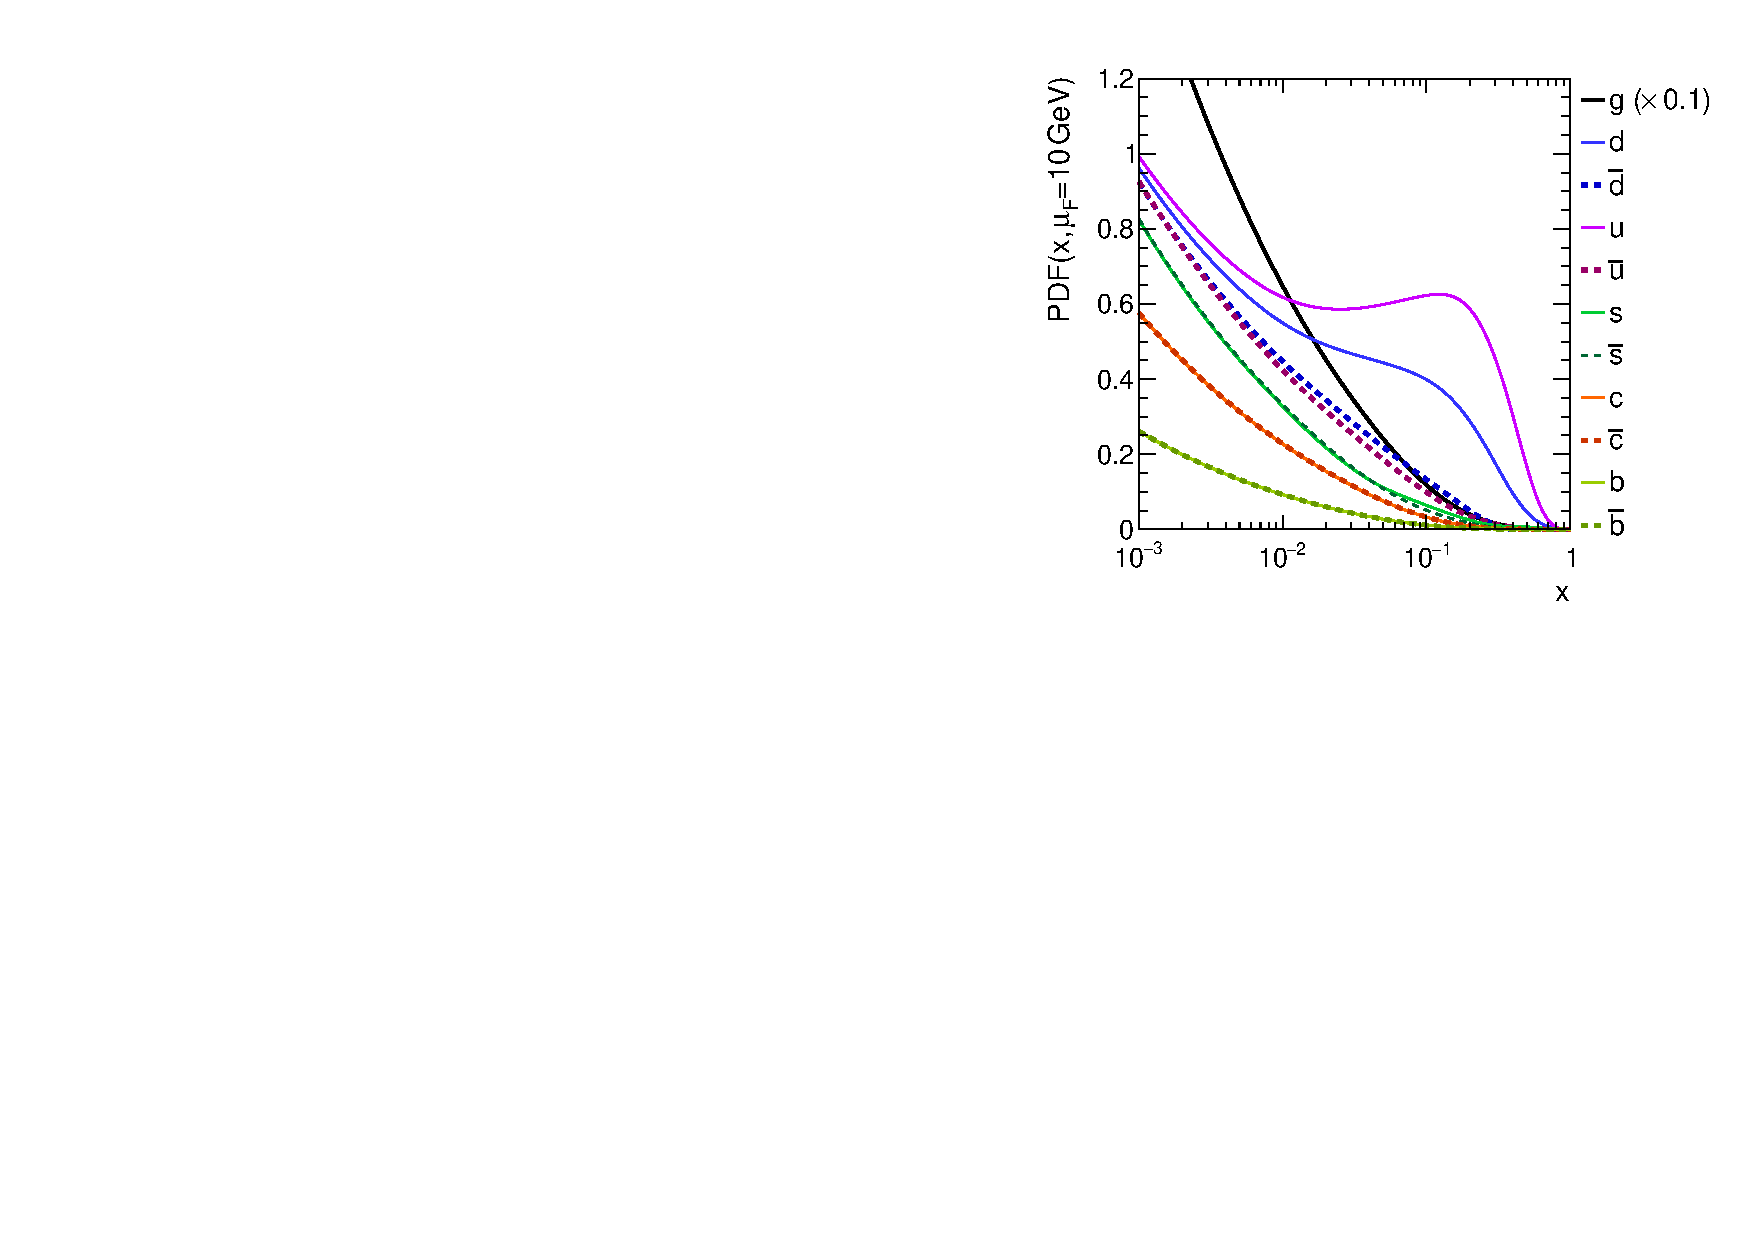
\includegraphics[width=0.49\textwidth]{figures/theory/nnpdf_q10.pdf}}\hspace{0.01\textwidth}
\subfloat[]{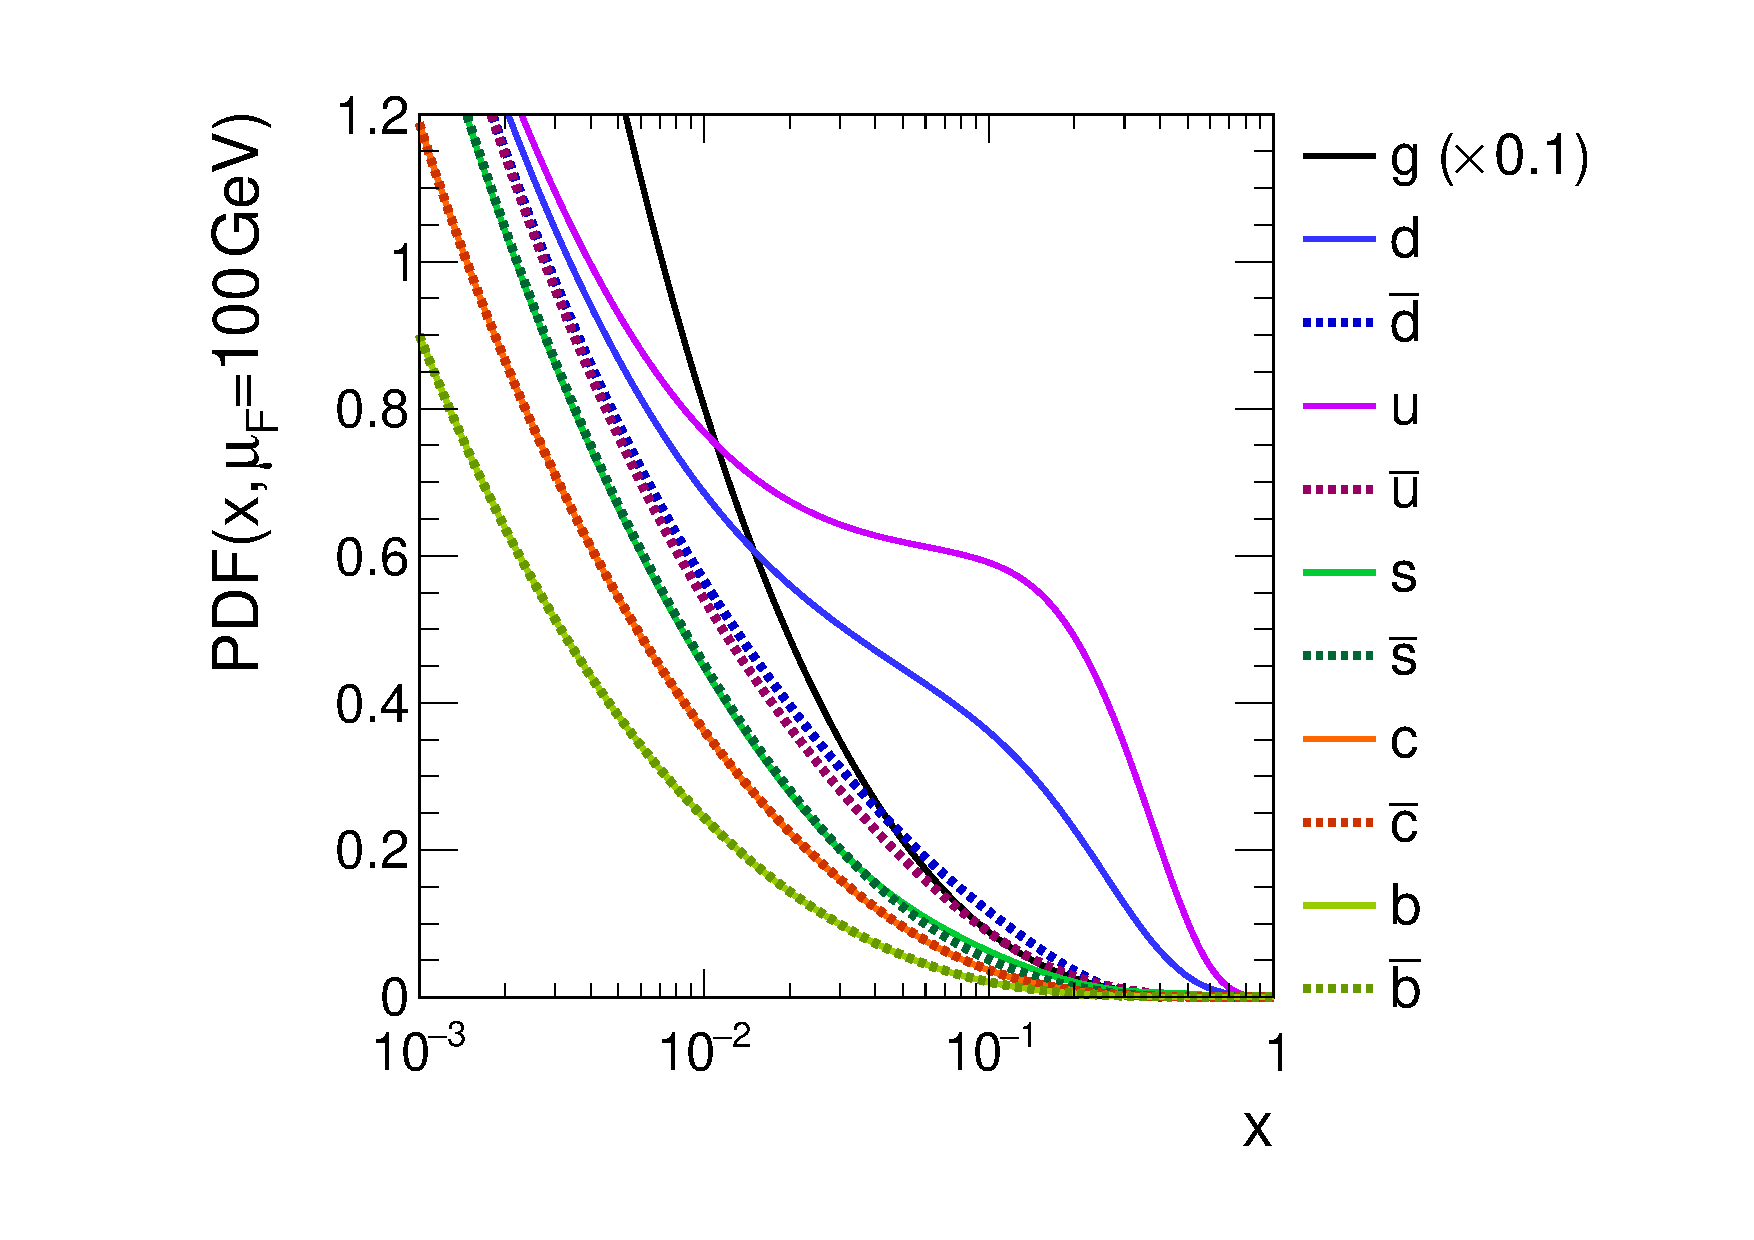
\includegraphics[width=0.49\textwidth]{figures/theory/nnpdf_q100.pdf}}
}

At high energies, quantum fluctuations lead to divergences as well. In order to let a theory still describe the experimental energy regime, physical quantities are redefined at the so-called ``renormalization scale'' $\mu_\mathrm{R}$. This leads to a ``running'' behavior of the coupling constants as a function of $\mu_\mathrm{R}$. Beyond this scale, high energy effects such as loop corrections to propagators~(so-called ``self-energy'') have been absorbed in the physical quantities through renormalization of the fields. In particular, the running behavior of the strong coupling constant is found to be 

\begin{equation}
\as(\mu_\mathrm{R})=\frac{\as(\mu_{0}^{2})}{1+\as(\mu_\mathrm{0}^2)\cdot\tfrac{33-2\cdot n_f}{12\pi}\cdot\ln\Big(\tfrac{|\mu_\mathrm{R}^2|}{\mu_{0}^{2}}\Big)}
\end{equation}

where $n_f$ denotes the number of quarks and $\mu_{0}$ is a reference scale where the coupling is known from measurements, e.g. $\mu_{0}=m_\mathrm{Z}$. The world average of the strong coupling constant $\as=g/(4\pi^2)$ at the $\mathrm{Z}$~boson mass is currently estimated to be $\as(m_\mathrm{Z})=0.1181\pm0.0011$~\cite{Olive:2016xmw}. 

Quarks can be treated as ``asymptotically free'' since the strong coupling decreases towards larger energies. On the other hand, following the behavior of $\as(\mu^2_\mathrm{R})$ towards lower energies, a limit $\Lambda_\mathrm{\gls{qcd}}\approx 200~\MeV$ is found at which $\as$ becomes even larger than one. Below such energies, perturbative calculations of observables can no longer be performed~(see Sec.~\ref{sec:theory-observables}). 





%##############################################
\section{Observables}
%##############################################
\label{sec:theory-observables}

A particle scattering process or decay is characterized by the initial and final particles as well as the interactions between them. Experimental observables are inclusive and differential cross sections as well as decay rates which can be calculated using perturbation theory. 

The cornerstone of such a calculation is the so-called \gls{smatrix} which describes the transition of a system from an initial to a final multiparticle state. In the Heisenberg picture, the time evolution of such a system is given by the Dyson series

\begin{align}
\mathcal{S}&=\mathrm{T}\Big[\exp\Big(-i\int\mathrm{d}^{4}x~\mathcal{H}_\mathrm{int}(t)\Big)\Big]\\
&=\sum_{n=0}^{\infty}\frac{(-i)^{n}}{n!}\int_{-\infty}^{\infty}\mathrm{d}^{4}x_{1}\ldots \int_{-\infty}^{\infty}\mathrm{d}^{4}x_{n}~\mathrm{T}\Big[\mathcal{H}_\mathrm{int}(t_{1})\ldots\mathcal{H}_\mathrm{int}(t_{n})\Big] \label{eq:theory-dyson-series}
\end{align}

where particle interactions are described within the non-free part of the Hamiltonian density $\mathcal{H}_\mathrm{int}=\mathcal{H}-\mathcal{H}_\mathrm{free}$. The operator $\mathrm{T}$ ensures that products of $\mathcal{H}_\mathrm{int}(t_{i})$ are ordered by time. The transition amplitude from an initial state to a final state with particles $\psi_i^\mathrm{in/out}$ respectively can hence be calculated using

\begin{align}
\mathcal{A}_\mathrm{in\to out}&=\langle\psi_{1}^\mathrm{out}\ldots\psi_{N^{\prime}}^\mathrm{out}\,|\,\mathcal{S}\,|\,\psi_{1}^\mathrm{in}\ldots\psi_{N}^\mathrm{in}\rangle \\
&=\langle\psi_{1}^\mathrm{out}\ldots\psi_{N^{\prime}}^\mathrm{out}\,|\,\psi_{1}^\mathrm{in}\ldots\psi_{N}^\mathrm{in}\rangle+i\mathcal{M}\,(2\pi)^{4}\delta^{4}\big(\Sigma p^\mathrm{in}_{i}-\Sigma p^\mathrm{out}_{j}\big)
\end{align}

where $\mathcal{M}$ captures the interaction terms at all orders of the perturbative series. If $\mathcal{H}_\mathrm{int}>1$ the series does not converges and one says the problem is not solvable perturbatively. Exemplary, the ground states of hadrons can not be calculated perturbatively because of the running of the strong coupling constant. An alternative approach is required. This problem was solved using lattice gauge theory~\cite{Durr:2008zz}.

The decay rate $\mathrm{d}\mathrm{N}/\mathrm{d}t=\Gamma\cdot\mathrm{N}$ of an unstable particle can be calculated from the width $\Gamma$ which is given by

\begin{align}
\Gamma&=\frac{1}{2m}\sum_\mathrm{out}\int\,\big|\,\mathcal{M}(\mathrm{in}\to\mathrm{out})\,\big|^2\mathrm{d}\Phi^\mathrm{out}\\
\mathrm{d}\Phi^\mathrm{out}&=(2\pi)^{4}\delta^{4}\big(\Sigma p^\mathrm{in}_{i}-\Sigma p^\mathrm{out}_{j}\big)~\prod_{j}\int\frac{\mathrm{d}^{3}~\vec{p}^\mathrm{~out}_{j}}{(2\pi)^{3}2E_{j}^\mathrm{out}}
\end{align}

where $\mathrm{d}\Phi^\mathrm{out}$ integrates over the phase space spanned by the outgoing particle momenta. The $\delta$ function ensures conservation of momentum and energy between the initial and final state. For a decay into a specific final state $f$ one defines the branching ratio as $\mathcal{B}(X\to f)=\Gamma(X \to f)/\sum\Gamma(X \to\mathrm{any})$ where $\sum_{f}\mathcal{B}(X \to f)=1$.

For a scattering process, the cross section $\sigma$ is defined as the number of interactions per unit density~($\rho=1$) given a flux $L=\rho v$ of incoming particles with velocity $v$. It is usually denoted in the unit ``barn''~[$\mathrm{b}$] which is defined as $1~\mathrm{b}\equiv 10^{-28}~\mathrm{m}^{2}$.  The number of interaction events per time is given by $\mathrm{d}N/\mathrm{d}t=L\sigma$. The flux $L$ is commonly referred to as luminosity.

For a collider experiment with beam energies $E_{i}$ and velocities $\vec{v}_{i}$ one finds the cross section as 

\begin{equation}
\sigma=\frac{1}{|\vec{v}_1-\vec{v}_2|}\frac{1}{4E_{1}E_{2}}~\int\,\big|\,\mathcal{M}(\mathrm{in}\to\mathrm{out})\,\big|^{2}~\mathrm{d}\Phi^\mathrm{out}. \label{eq:theory-xsec-calculation}
\end{equation}

In the case of hadron-hadron collisions, Eq.~\ref{eq:theory-xsec-calculation} only calculates the partonic cross section. Exemplary, for the process $\mathrm{pp}\to X$ the total cross section can be calculated as

\begin{equation}
\sigma(\mathrm{pp}\to X)=\sum_{i,j}\iint\mathrm{d}x_{1}\,\mathrm{d}x_{2}~\mathrm{PDF}(x_{1},f_{i})\,\mathrm{PDF}(x_{2},f_{j})\,\sigma(f_{i}f_{j}\to X)
\end{equation}

where additional summations and integrations over the \glspl{pdf} are required to account for the individual contributions per parton flavor $f_{i}$ and per momentum fraction $x_{i}$.


Calculations of observables can be written in terms of the number of interaction vertices contributing to $\mathcal{M}$ originating from the perturbative series~(Eq.~\ref{eq:theory-dyson-series}). This allows to the expand an observable as a power series in terms of the coupling constant $\alpha$ as

\begin{equation}
\sigma=\sigma_\mathrm{\glsunset{lo}\gls{lo}}\Big(1+\frac{\alpha}{2\pi}\cdot\sigma_\mathrm{1}+\big(\frac{\alpha}{2\pi}\big)^2\cdot\sigma_{2}+\big(\frac{\alpha}{2\pi}\big)^{3}\cdot\sigma_{3}+\ldots\Big).
\end{equation}

\todo{what is NNLL?}

Depending at which term the series is cut off one speaks of \glsreset{lo}\gls{lo}, \gls{nlo}, or \gls{nnlo} accuracy in $\alpha$. In general, it is desirable to calculated observables beyond \gls{lo}. Predictions including higher order corrections tend to be less affected by theoretical uncertainties which originate from a variation of the chosen renormalization and factorization scales\footnote{Partonic \gls{lo} cross sections can only be monotonous functions of $\mu_\mathrm{R}$ since $\sigma\propto\alpha(\mu_\mathrm{R})$. Hence, an uncertainty due to a scale variation can be even considered meaningless.}.

From the unitarity $\mathcal{S}^{\dagger}\mathcal{S}=1$ of the \gls{smatrix} the optical theorem can be derived. It states that the imaginary part of a scattering amplitude $\mathcal{M}(i\to f)$ is directly related to the scattering amplitude of producing all possible intermediate particles $\chi$ from the initial times the final state $\sum_{X}\mathcal{M}^\dagger(i\to \chi)\mathcal{M}(f\to \chi)$. This leads to general constraints on the total cross section. For example, the scattering amplitude of a $2\to2$ process can be expressed via the optical theorem as

\begin{align}
2\,\mathrm{Im}\Big(\mathcal{M}(\psi_{1}\psi_{2}\to\psi_{1}\psi_{2})\Big)&=4E_1E_2\,|v_1-v_2|\,\sigma_\mathrm{tot}(\psi_{1}\psi_{2}\to\mathrm{any})\\
&=\sum_{\chi}\beta_{\chi}\int\frac{\mathrm{d}\cos\theta}{16\pi}\,\big|\mathcal{M}(\psi_{1}\psi_{2}\to \chi)\big|^2
\end{align}

where $\beta_{\chi}$ is given by the integral over the final state phase space.

Since the total cross section is at least as big as the scattering cross section one finds that the matrix elements are bound and cannot be arbitrary large. Exemplary bounds on effective four-fermion interactions (in the context of dark matter production) are derived in Ref.~\cite{Endo:2014mja}. 

Hypothetical, a theory may describe experimental data well but still violates the unitarity bound at higher energies beyond the experimental probing capabilities. Such a case would hint towards a new physics model which restores unitarity by introducing new particles or interactions at energies before it is violated. This is called \gls{uv} completion. A unitarity-violating theory may just reflect the low energy limit of an unknown \gls{uv}-complete theory within the experimental energy regime. Exemplary,  the $\mathrm{W}^{\rmplus}\mathrm{W}^{\rmminus}\to\mathrm{W}^{\rmplus}\mathrm{W}^{\rmminus}$ scattering amplitude would grow as $\mathcal{M}\sim s/m_\mathrm{W}^2$ if there is no Higgs boson and eventually violate unitarity at $\sqrt{s}\approx1~\TeV$.


%##############################################
\section{Open questions}
%##############################################

The \gls{sm} is believed to be not the final theory describing fundamental interactions. In the following, some of its problems are discussed briefly.

\begin{description}
\item[Gravity] The \gls{sm} cannot describe gravitational interactions. Its mediator, the graviton, would have to be a spin~2 boson which however leads non-renormalizable divergences. However, at energy scales reached by colliders, it is fine to ignore gravitational interactions since those become only comparable in strength to the electroweak and strong interactions at the Planck scale $\Lambda_\mathrm{P}\approx10^{18}~\GeV$. 
\item[Naturalness] A large correction to the bare Higgs boson mass originates from top quark loops due to Yukawa interactions. Those need to be absorbed by the physical mass through renormalization. The resulting mass can be written as $m^{2}_\mathrm{H}\approx m_\mathrm{bare}+\lambda_\mathrm{t}^{2}\mu^2/(16\pi^2)$. If the \gls{sm} is valid up to the Planck scale $\mu=\Lambda_\mathrm{P}$, it would require an extraordinary fine-tuning of the bare Higgs mass in order to cancel this large correction. Such a coincidence is considered to be not very ``natural''.
\item[Dark matter and dark energy] Cosmological observations of rotation speeds of galaxies, mapping of matter distributions through micro-lensing, and acoustic oscillations in the cosmic microwave background suggest that there exists a yet unidentified kind of matter, called ``dark matter''. It seems to interact only through gravity with ordinary matter. A yet even more puzzling building block of the universe which missing from the \gls{sm} is dark energy. It is a crucial ingredient to describe the expansion of the universe for which the universe has to be composed of 74\% dark energy, 22\% dark matter, and 4\% ordinary baryonic matter of which only 0.4\% is even compact.

\end{description}

